%%% arquitetura - geral
\begin{frame}{Arquitetura - Geral}

\vspace*{-3em}

\begin{itemize}
	\item \textbf{API}: desenvolvida em Typescript e executada sobre Node.js;
	\item \textbf{Aplicação móvel}: desenvolvida em Kotlin para o sistema operativo Android;
	\item \textbf{Aplicação \textit{web}}: desenvolvida utilizando React para clientes \textit{browser}.
\end{itemize}

\centering
\scalebox{0.30}{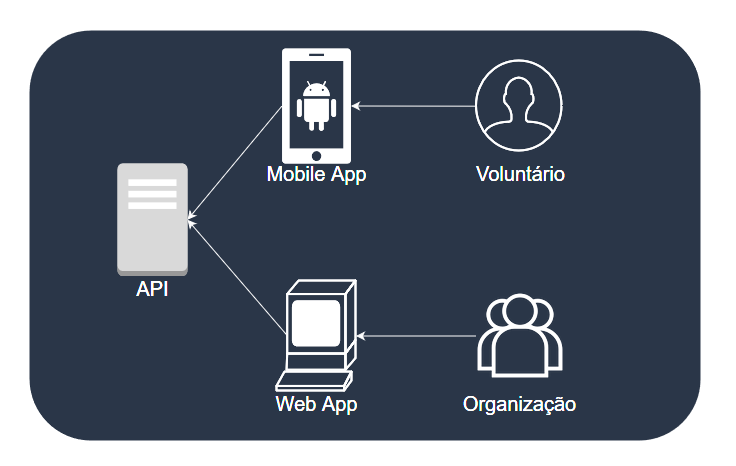
\includegraphics{Figures/architecture-general}}\\

{\small Arquitetura geral do projeto.}

\end{frame}

%%% api - conceito e funcionalidade
\begin{frame}{API - Conceptualização e Funcionalidades}

\vspace*{-4em}

\begin{itemize}
	\item Entidades:
	\begin{itemize}
		\item \textbf{Voluntário}: indivíduo participante da ação;
		\item \textbf{Organização}: entidade que organiza ação;
		\item \textbf{Evento}: ação de voluntariado;
		\item \textbf{\textit{Post}}: meio de interação entre utilizadores.
	\end{itemize}

	\vspace*{1em}

	\item Funcionalidades:
	\begin{itemize}
		\item adicionar e alterar entidades;
		\item assegurar interação entre utilizadores;
		\item permitir que organizações possam verificar e obter contatos de voluntários interessados.
	\end{itemize}
\end{itemize}

\end{frame}

%%% api - arquitetura
\begin{frame}{API - Arquitetura}

\vspace*{-3em}

\begin{itemize}
	\item \textbf{Controladores}: definem \textit{endpoints} e lidam com pedidos HTTPS;
	\item \textbf{Serviços}: implementam a lógica de negócio;
	\item \textbf{Repositórios}: interagem com a base de dados.
\end{itemize}

\centering
\scalebox{0.20}{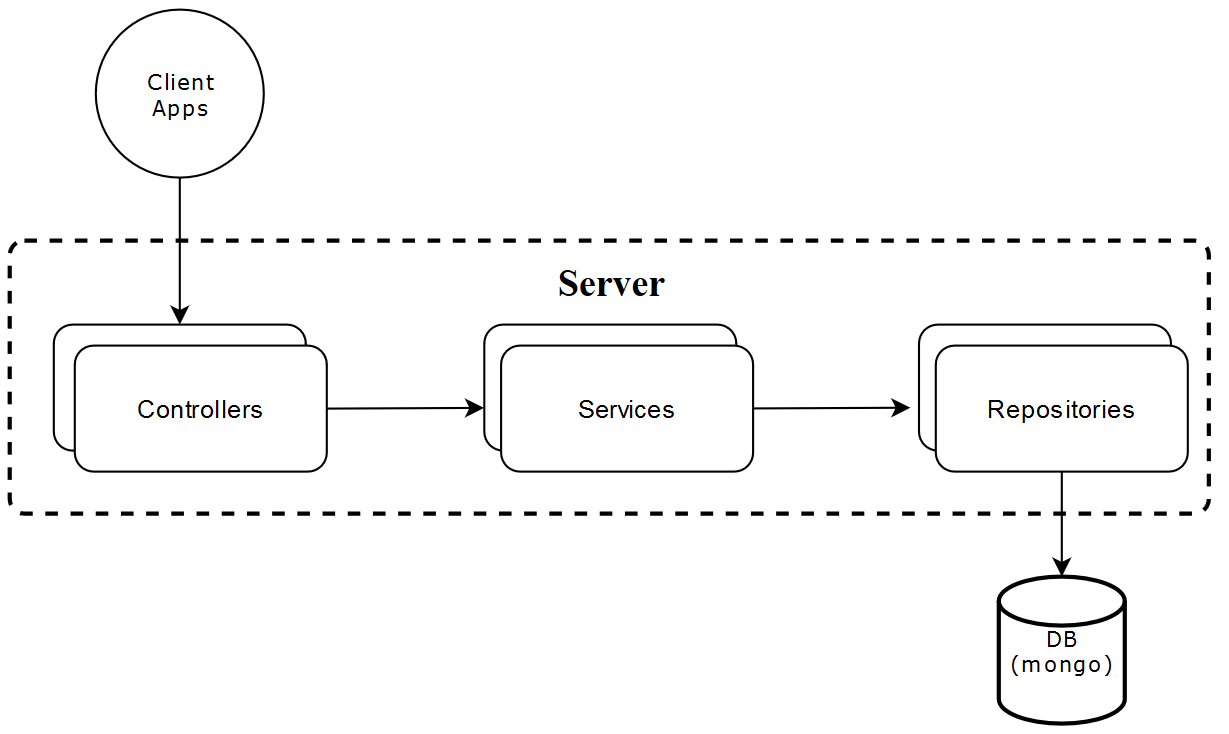
\includegraphics{Figures/api_architecture}}\\
{\small Arquitetura da API.}

\end{frame}

%%% app movel - funcionalidade
\begin{frame}{Aplicação Móvel - Funcionalidades}

\vspace*{-3em}

\begin{itemize}
	\item Consultar \textbf{voluntários, organizações, eventos e posts};
	\item permitir o registo e autenticação de voluntários através da aplicação;
	\item possibilitar aos utilizadores autenticados interagir com a plataforma (realização de \textit{posts}, seguimentos de outros utilizadores, etc.).
\end{itemize}

\end{frame}

%%% app movel - arquitetura
\begin{frame}{Aplicação Móvel - Arquitetura}
	
\vspace*{-4em}
	
\begin{itemize}
	\item \textbf{Ecrãs}: definem a interface de utilizador e o tratamento de operações de \textit{input}; Para cada ecrã, existe associado um ViewModel;
	\item \textbf{API}: funciona como \textit{proxy} da \textit{web} API.
\end{itemize}	

\centering
\scalebox{0.40}{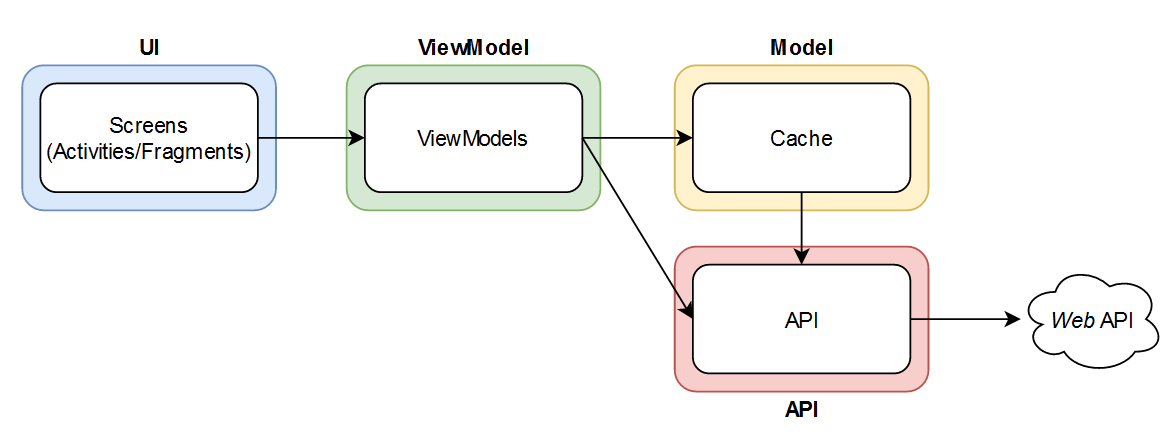
\includegraphics{Figures/mobile_app_architecture}}\\

{\small Arquitetura da aplicação móvel.}

\end{frame}

%%% api - arquitetura
\begin{frame}{Aplicação \textit{web}}

\vspace*{-2em}

\centering
\scalebox{0.35}{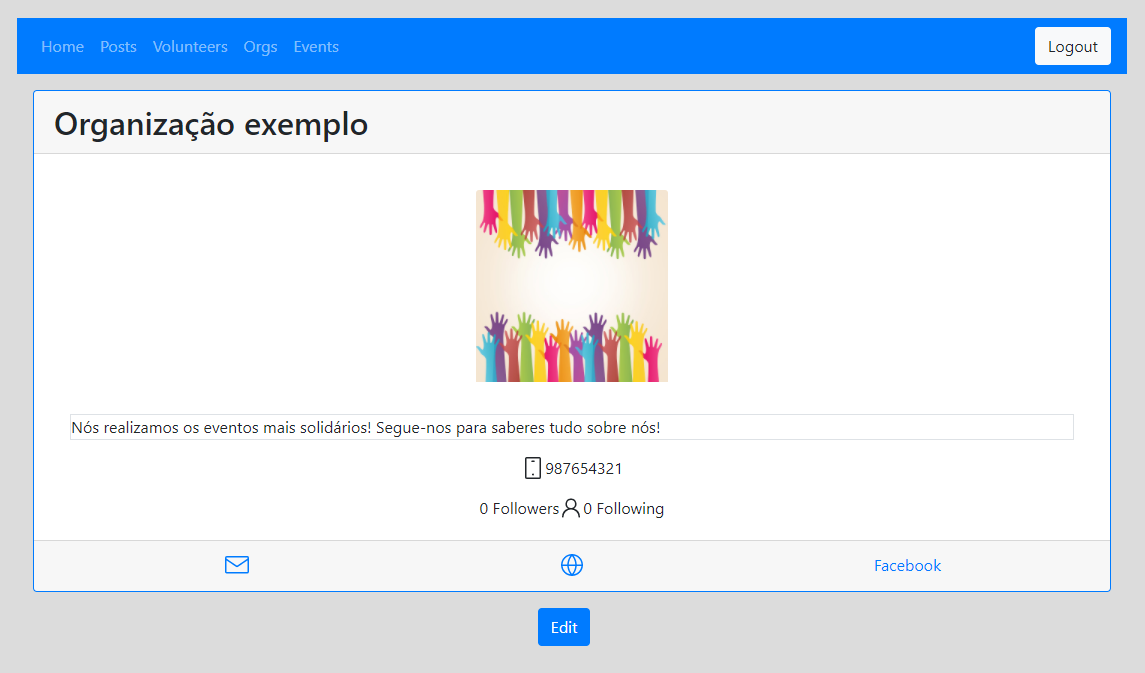
\includegraphics{Figures/web_app_dashboard}}\\

{\small \textit{Dashboard} da aplicação.}

\end{frame}

%%% api - arquitetura
\begin{frame}{Aplicação \textit{web} - Arquitetura}
	
\vspace*{-3em}
	
\begin{itemize}
	\item \textbf{Classe Principal}: instancia serviços da API e define roteamento da aplicação;
	\item \textbf{Componentes}: definem a interface de utilizador, incluindo o tratamento de operações de \textit{input};
	\item \textbf{API}: contém implementação de serviços utilizados para aceder à \textit{web} API.
\end{itemize}		

\centering
\scalebox{0.4}{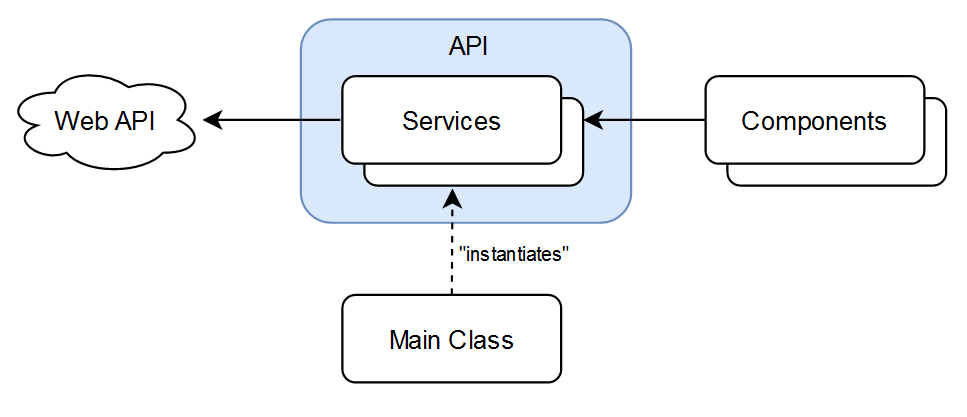
\includegraphics{Figures/web_app_architecture}}\\

{\small Arquitetura da aplicação \textit{web}.}

\end{frame}